%----------------------------------------------------------------------------------------
%	PACKAGES AND DOCUMENT CONFIGURATIONS
%----------------------------------------------------------------------------------------

\documentclass{article}


\usepackage{graphicx} % Required for the inclusion of images
\usepackage{subfigure} % Required for the inclusion of images
%\usepackage{natbib} % Required to change bibliography style to APA
\usepackage{amsmath} % Required for some math elements
\usepackage{pdfpages}


%\usepackage{times} % Uncomment to use the Times New Roman font

%----------------------------------------------------------------------------------------
%	DOCUMENT INFORMATION
%----------------------------------------------------------------------------------------

\title{\textbf{Project 1: Optimizing the Performance of a Pipelined Processor}} % Title

\author{000, x, x-email \\
        001, y, y-email \\
        002, z, z-email } % Author name and email

\date{\today} % Date for the report

\begin{document}


\maketitle % Insert the title, author and date

\section{Introduction}

[In this section you should briefly introduce the task in your own words, and what you’ve done in this project. A simple copy from project1.pdf is not permitted.] \\

\noindent[You should also list the arrangement of each member here. For example, you can write, “student-x finished part A and B, student-y finished part C and student-z finished the report” (of course we suggest each student to make contributions to coding tasks.)]

\section{Experiments}

[This is the main part of your report. It includes three parts and in each part, you need to write concretely, logically but not in full details.]


\subsection{Part A}

\subsubsection{Analysis}

[In this part, you should give an overall analysis for the task, like difficult point, core technique and so on.]

\subsubsection{Code}

[In this part, you should place your code and make it readable in Microsoft Word, please. Writing necessary comments for codes is a good habit.]

\subsubsection{Evaluation}

[In this part, you should place the figures of experiments for your codes, prove the correctness and validate the performance with your own words for each figure’s explanation.]

\subsection{Part B}

\subsubsection{Analysis}

[In this part, you should give an overall analysis for the task, like difficult point, core technique and so on.]

\subsubsection{Code}

[In this part, you should place your code and make it readable in Latex, please. Writing necessary comments for codes is a good habit.]

\subsubsection{Evaluation}

[In this part, you should place the figures of experiments for your codes, prove the correctness and validate the performance with your own words for each figure’s explanation.]

\subsection{Part C}

\subsubsection{Analysis}

   \par In this part, we are required to optimize the performance of a function ncopy, which copies the data from source address to destine address and return the number of positive integers contained in the source. And to achieve this goal, optimization of both algorithm and hardware is allowed. So, this part is a test of our overall capability of pipeline architecture.
    \par  The performance of the function is evaluated with CPE, so what we need to do is to reduce average CPE as more as possible. The difficulties lie in several aspects below, and we have also figured out the answer.
\begin{enumerate}
    \item
	What makes the function perform poorly? A: Great number of branch instructions, high cost of computation involving immediate integers and stall penalty from load-read instructions. We are not talking about misprediction penalty of conditional branches but just the proportion of branch instructions that would cost a lot of cycles.
    \item
	How can we reduce branch instructions, computation cost and stall penalty? A: Reduce instructions of conditional branches to improve our algorithm, add new instruction(s) to increase support for immediate computation and adjust sequence of some instructions.
    \item
	What should we do in software layer? A: Modify ncopy.ys, and apply technique of loop unrolling to reduce number of branch instructions, use instruction(s) that supports immediate computation better when necessary and adjust sequence of some instructions that would cause a data hazard.
    \item
	What should we do in hardware layer? A: Modify pipe-full.hcl, and implement logic that supports immediate computation, that is iaddl. (Apart from iaddl, ileave is also implemented here according to the requirement but it is found to be of no use in this part.)
Now we will elaborate what we do here.
\end{enumerate}
	   \par Firstly, loop unrolling. Technique of loop unrolling reduces the number of branch instructions and thus reduce the number of instructions to execute. We have a loop that performs ncopy of 16 elements. In the primitive version of ncopy every time a number is copied there would be a check whether the loop should be over. Thus, we reduce the number of instructions by 15 every 16 elements, which also means that the CPE could be decreased by about 15/16 with technique of loop unrolling. Also, we need to tie up some loose ends. To achieve better performance, after the 16-element loop, we do the ncopy work with 8, 4, 2 and 1 element(s) successively if there are that many elements left.
	   \par Secondly, use iaddl for immediate computation. Decreasing of len and increasing of count, p\_src and p\_dst are involved with immediate operands. We could have CPE decreased by 2 with this step.
	   \par Thirdly, avoid load-read stall penalty. It is easy to find a“mrmovl x1, x2” instruction followed by a “rmmovl x2, x3” instruction, which intends to copy *p\_x1 to *p\_x3. But since mrmovl is a load instruction and rmmovl needs to read the same register. So, codes like this would cause a penalty of one cycle. In other words, by inserting some other instructions into the two instructions can decrease the CPE approximately by 1.
	   \par Fourthly, implementation of iaddl and ileave. Detailed descriptions of iaddl and leave can be seen in the beginning part of seq-full.hcl and pipe-full.hcl. (Although we are talking about implementation of pipeline processor, but the operations of the two instructions are similar to that of a sequence processor) . iaddl, which adds an immediate operand to a register, can be accomplished by combination of irmovl and addl. leave, which decrease stack pointer and load data to base pointer register memory addressed by itself, can be accomplished y combination of mrmovl and popl. Inspired by instructions similar to them, we could modify the hcl file properly. Here are some further details. Iaddl: instr\_vali, need\_regids, need\_valC, d\_srcB = D\_rB, d\_dstE = D\_rB, aluA = valC, aluB = valB, set\_cc. leave: instr\_vali, need\_regids, d\_srcA = REBP, d\_dstE = RESP, d\_dstM = REBP, aluA = E\_valA, aluB = 4, mem\_addr = M\_valA, mem\_read, F\_stall, D\_stall, D\_bubble, E\_bubble. Using iaddl instruction can also reduce CPE by about 2.\\


\subsubsection{Code}


    \textbf{Beginnning of ncopy.ys} \\
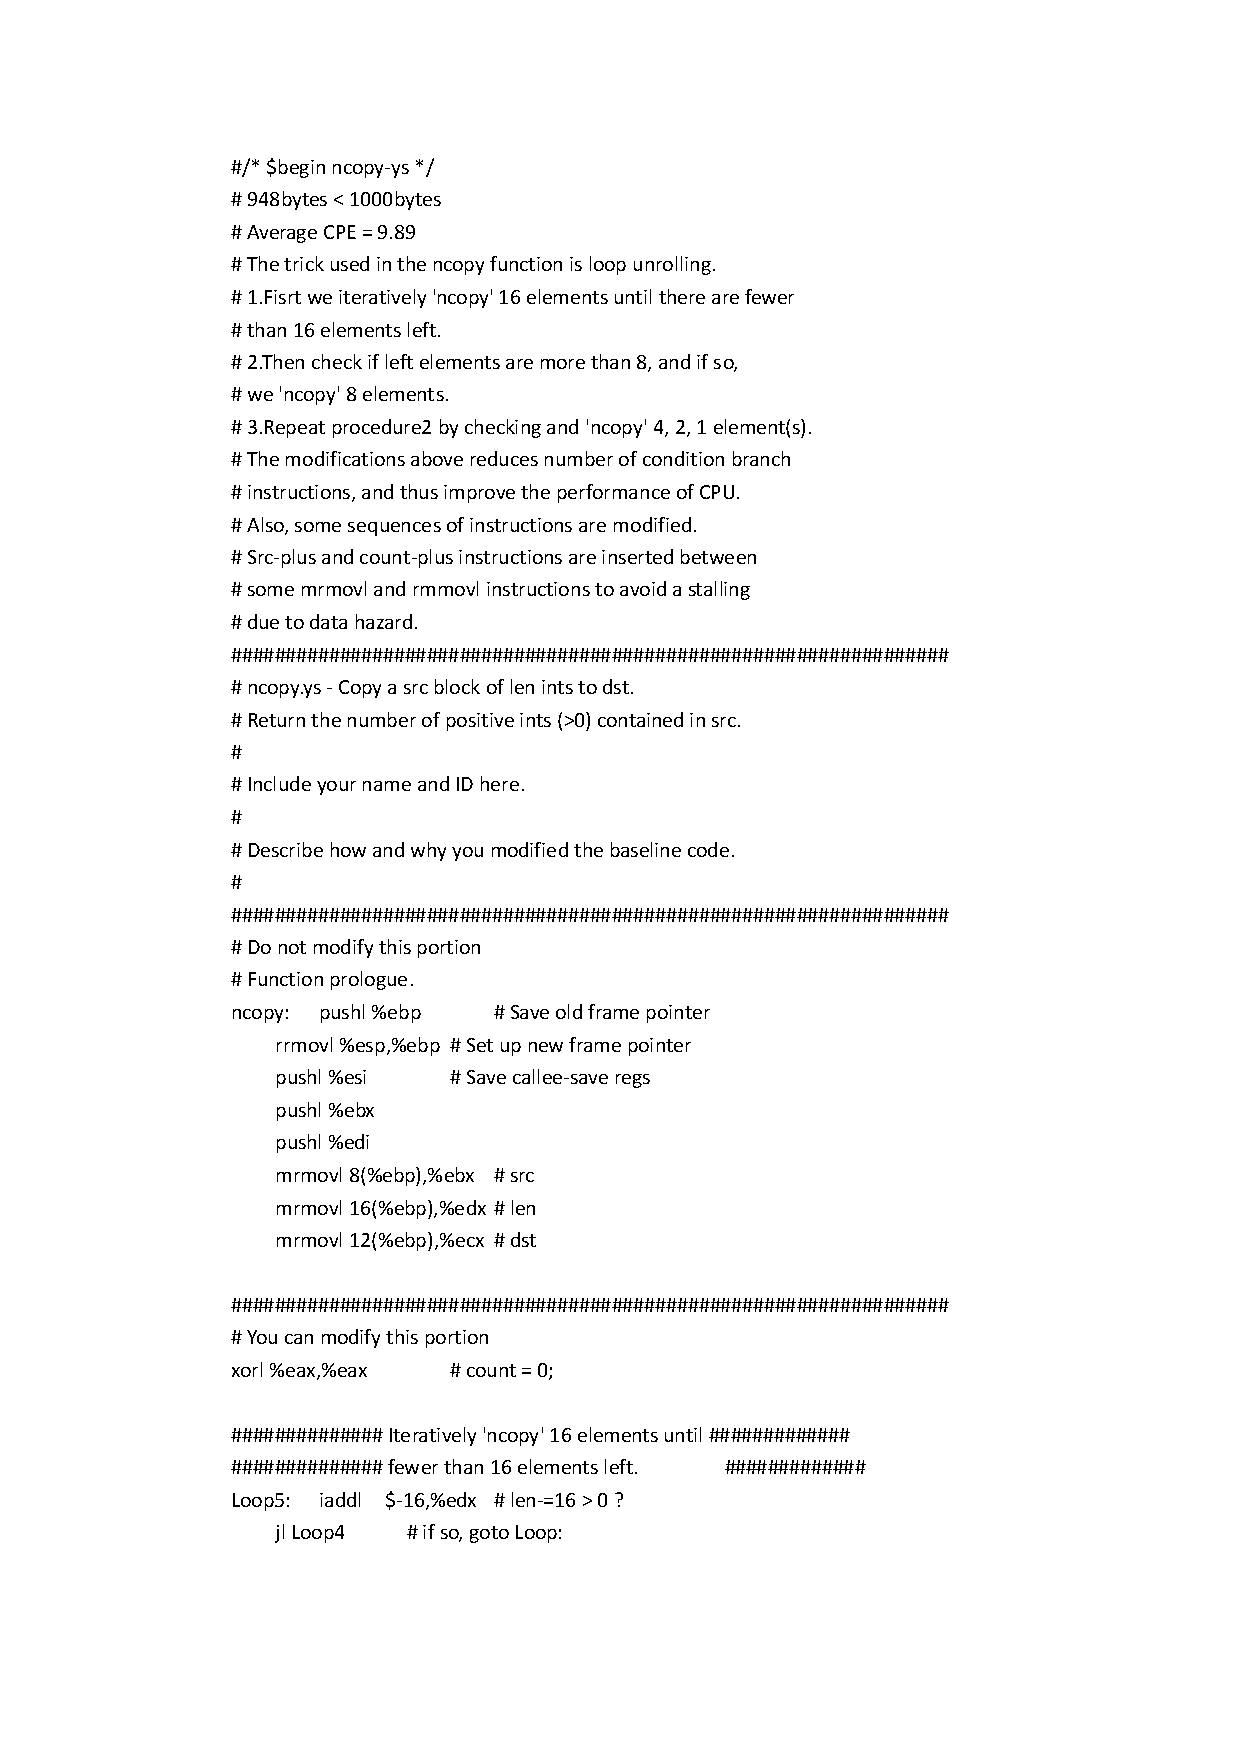
\includepdf[pages={1,2,3,4,5,6,7}]{ncopy.pdf}
\textbf{Ending of ncopy.ys} \\
\\
\textbf{Beginning of pipe-full.hcl} \\

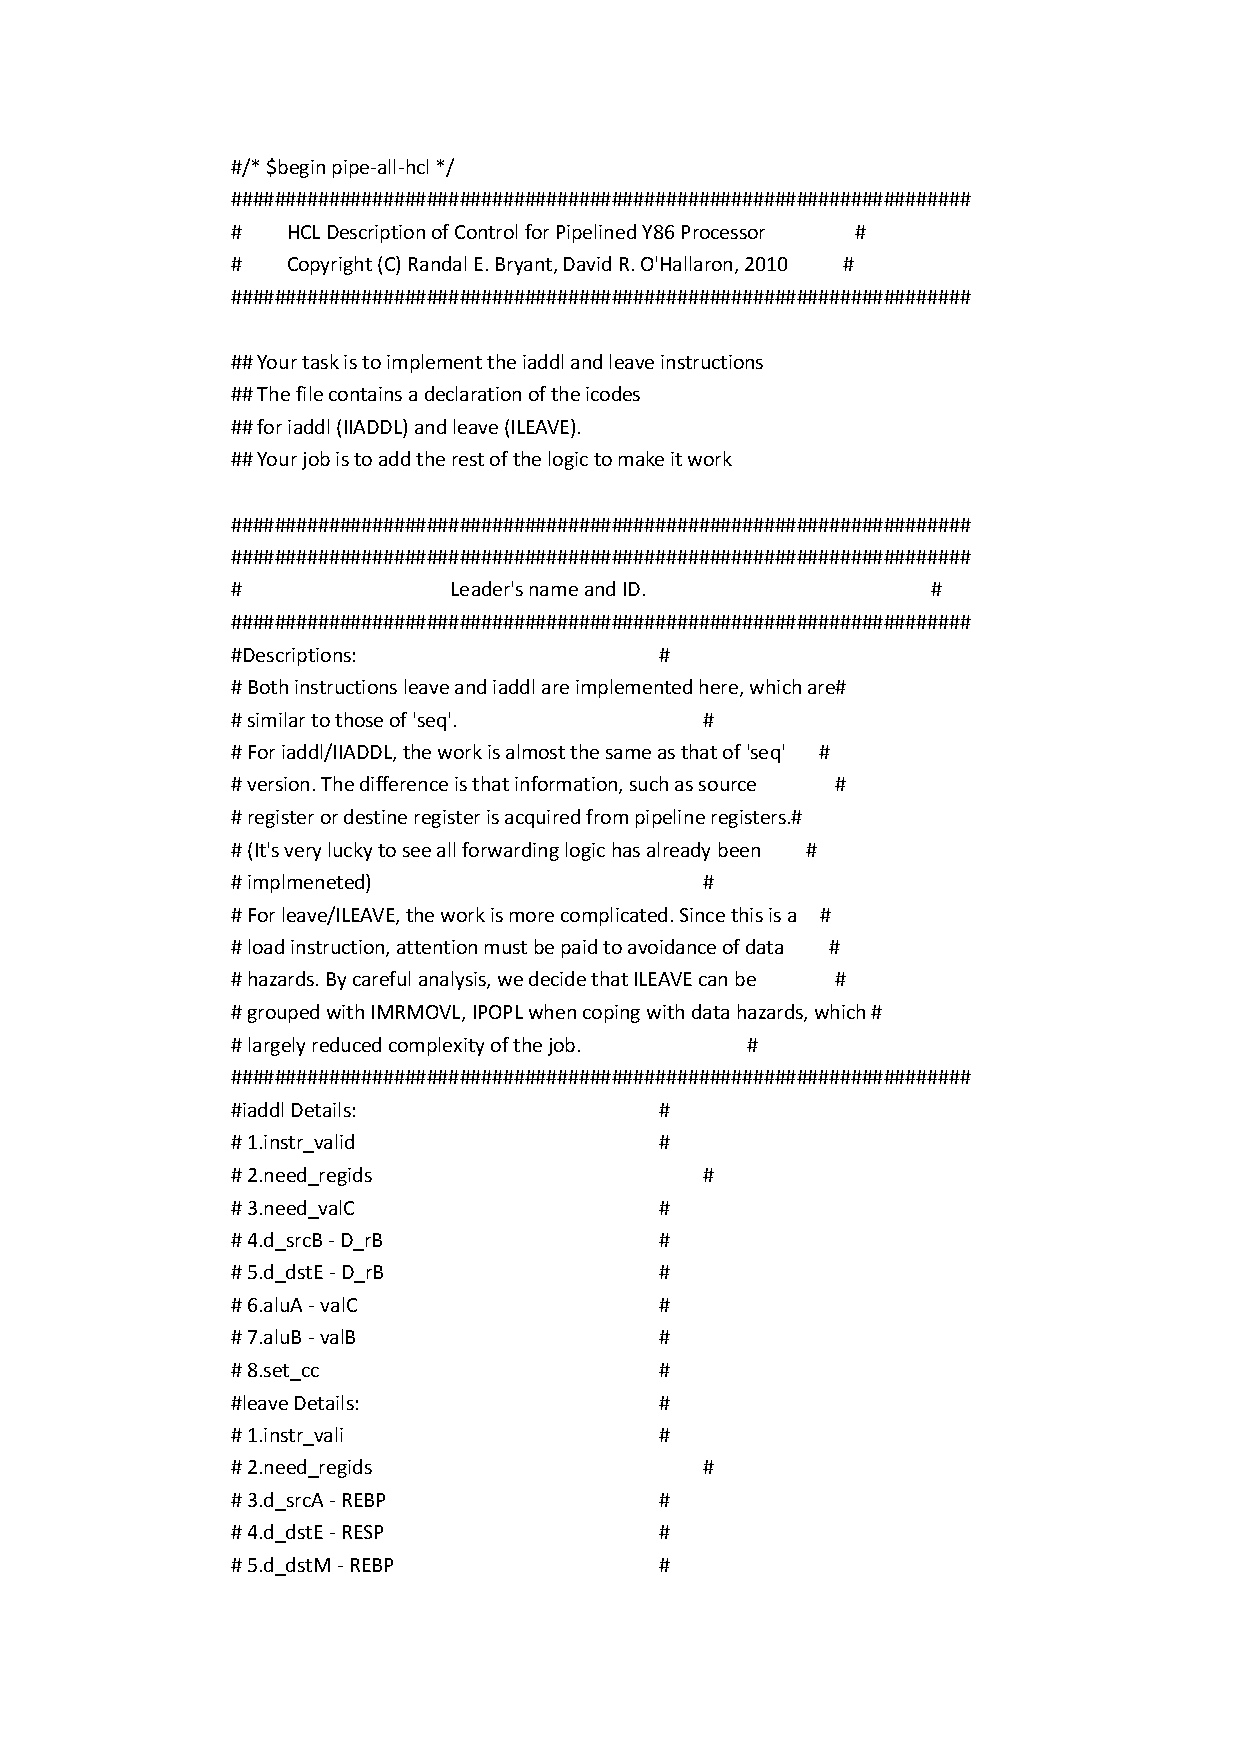
\includepdf[pages={1,2,3,4,5,6,7,8,9,10}]{pipe-full.pdf}

\textbf{Ending of pipe-full.hcl} \\



\subsubsection{Evaluation}
    Now, we are going to evaluate the result of part C.\\
\begin{enumerate}

  \item Firstly, as shown in the figure below, our modifications do not change the correctness of existing instructions.\\
  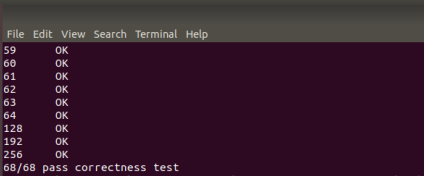
\includegraphics[width=0.95\textwidth]{pipe_correctness.png}
  \item Secondly, as shown in the figure below, the ncopy file is 948bytes, less than the required 1000bytes. \\
  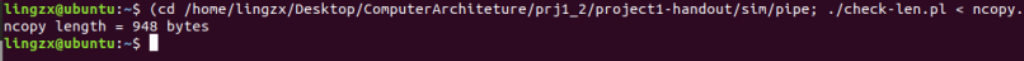
\includegraphics[width=0.95\textwidth]{pipe_checklen.png}
  \item Thirdly, as shown in the figure below, our implementation of iaddl and leave has survived all ISA checks.\\
  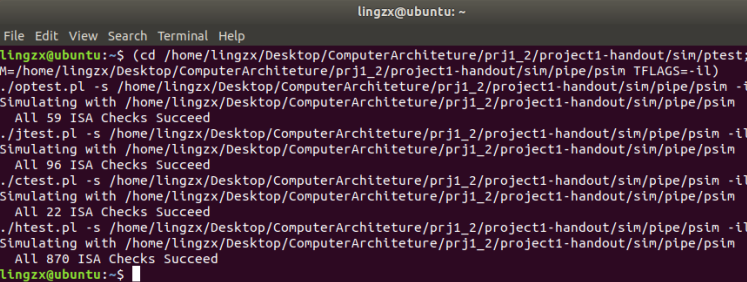
\includegraphics[width=0.95\textwidth]{pipe_ISACheck.png}
  \item Fourthly, as shown in the figure above, our ncopy function achives an average CPE of 9.89, less than 10.0, which means ncopy performs very well. As expected, the larger the number of elements is, the better the function performs. That is because when there are only several elements, loop unrolling and loose ends increase branch instructions; however, when the number is larger, the reduction of branch instructions caused by loop unrolling becomes remarkable.\\
  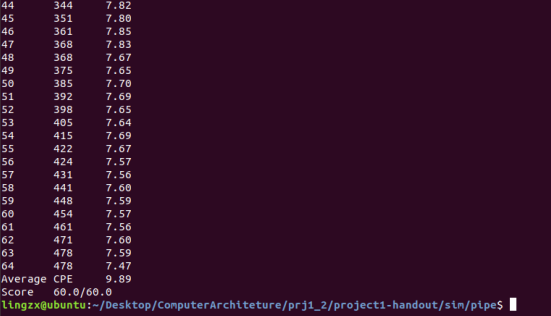
\includegraphics[width=0.95\textwidth]{pipe_CPE.png}
\end{enumerate}

\section{Conclusion}

\subsection{Problems}
There are many obstacles in the project. And we are going to share some here. \\
\begin{enumerate}

  \item Firstly, adjustment to new languages. You can never image how we feel when starting the project. It is just like language bombing. Both Y86 and HCL are new to us. And the related resources on the Internet are so poor that we have no idea how to start. However, after days of searching and thinking, we gradually adjust ourselves to the new languages. Y86 is similar to but much simpler than X86 and MIPS familiar to us. As for HCL, though more complex, the project does not require us to fully master it. It is enough if we just known how to make the logic clear. Besides, thanks to CSAPP, we can acquire a lot of related materials in the book. 
  \item Secondly, debugging assembly codes run by pipeline processor. It is amazingly difficult to debug our codes running by a pipeline processor. Just as the pipeline architecture is complex, the procedure of debugging is complex, too. The codes are not finished line by line. An instruction is finished in the M or WB stage and the next several instructions are already on the way. However, this does not both us in the end. Gradually, we learn to examine the contents of states and inputs of different stages and this exactly deepens our understanding of pipeline processors.
  \item Thirdly, understanding of stack pointer. This is exactly a detail problem. In this semester, we have read a lot of assembly codes but wrote little. The stack is used when passing arguments, saving registers and calling functions. As written in the given Y86 code examples, the convention is that, on entering a function, we save the base pointer(ebp), and copy the stack pointer(esp) to the base pointer. It takes us a long time to figure out why the address of the first argument is ebp+8. And finally, by carefully observing the contents of the stack, we found when esp is copied to ebp, the stack is pushed twice: one is to save the return address and the other is to save ebp. Also, on the same problem, we spend a long time to debug our rsum function just because we pass an argument when calling the function by pushing the stack BUT forgot to pop the stack to restore the stack pointer after the function is returned. 
\end{enumerate}

\subsection{Achievements}

\begin{enumerate}
  \item Firstly, it is great to see we have achieved an average CPE less than 10.0. This a result of our careful design of our logic and implementation. And all of us three members have contributed a lot in the process.
  \item Secondly, we have successfully implemented leave instruction. Leave is more complicated than iaddl, especially in the pipeline architecture because it involves necessary load-read hazard, but we have implemented it.
\end{enumerate}



%----------------------------------------------------------------------------------------


\end{document} 